%
% teil3.tex -- Beispiel-File für Teil 3
%
% (c) 2020 Prof Dr Andreas Müller, Hochschule Rapperswil
%
\section{Fraktale Bildkomprimierung
\label{ifs:section:teil3}}
\rhead{Fraktale Bildkomprimierung}
Mit dem Prinzip dieser IFS ist es auch möglich, Bilder zu komprimieren.
Diese Idee hatte der Mathematiker Michael Barnsley, welcher mit seinem Buch {\em Fractals Everywhere} einen wichtigen Beitrag zum Verständnis von Fraktalen geliefert hat.
Das Ziel ist, ein IFS zu finden, welches das Bild als Attraktor hat.
In diesem Unterkapitel wollen wir eine Methode dafür anschauen, wie sie in \cite{ifs:Rousseau2012} beschrieben ist.

Es ist wohl nicht falsch zu sagen, dass Ähnlichkeiten zur gesamten Menge, wie wir sie zum Beispiel beim Barnsley Farn gesehen haben, bei Bilder aus dem Alltag eher selten anzutreffen sind.
Ein IFS, wie wir es in \ref{ifs:subsection:IteratedFunktionensysteme} definiert haben, wird uns also nicht weiter helfen.
Anders sieht es mit partitionierten IFS (PIFS) \cite{ifs:pifs} aus.

In \ref{ifs:transformation} wurde definiert, dass die Kontraktionen $S_i$ bei IFS auf die gesamte Menge $E$ angewendet werden.
Bei einem PIFS wird der Attraktor in disjunkte Teilmengen aufgeteilt. 
Für jede dieser Teilmengen $R_i$ braucht es dann eine grössere Teilmenge, welche mit einer affinen Transformation eine zu $R_i$ ähnliche Menge bildet.
Wir müssen nicht mehr Ähnlichkeiten zum ganzen Bild finden, sondern nur zwischen Teilen des Bildes.
Doch wie finden wir das PIFS, welches das Bild als Attraktor hat?

\subsection{Das Kompressionsverfahren
\label{ifs:subsection:malorum}}
Wir beschränken das Verfahren für Graustufenbilder. Wie das Verfahren für Farbbilder verwendet werden kann, wird später erläutert.
Ein Graustufenbild kann man als Pixelraster mit einer $x$ und $y$ Achse verstehen.
Jedem dieser Pixel wird ein Grauwert zugeordnet.
Ein Bild ist also eine Funktion, die jedem Pixel einen Grauwert \(z = f(x,y)\) zuweist.

Wir suchen ein PIFS, welches das zu komprimierende Bild als Attraktor hat.
In einem ersten Schritt teilen wir das Bild in disjunkte benachbarte $b \times b$ Pixel-Quadrate auf. Diese Blöcke nennen wir Range-Blöcke der Menge $R=\{R_0,R_1,...R_m\}$. Diese sind als Raster im rechten Bild der Abbildung \ref{ifs:FIC} dargestellt.

Im nächsten Schritt teilen wir das Bild in alle möglichen $2b \times 2b$ Pixel-Quadrate auf. Diese sind die Domain-Blöcke der Menge $D = \{D_0,D_1,...D_n\}$. 
Im dritten und letzten Schritt wird für jeden Range-Block $R_i$ ein Domain-Block $D_j$ gesucht, welcher ihm am ähnlichsten ist.
Zwei Beispiele wie solche Domain-, und Range-Block Paare aussehen können, sehen wir in Abbildung \ref{ifs:FIC}

\subsubsection{Finden des ähnlichsten $D_j$}
Zuerst brauchen wir die Transformation 
\begin{align*}
	T_i(x,y,z) = 
	\begin{pmatrix}
		a_i & b_i & 0 \\
		c_i & d_i & 0 \\
		0 & 0 & s_i
	\end{pmatrix}
	\begin{pmatrix}
		x \\
		y \\
		z
	\end{pmatrix}
	+
	\begin{pmatrix}
		\alpha_i \\
		\beta_i \\
		g_i
	\end{pmatrix}
\end{align*}
um ein Element aus $D$ auf ein Element von $R$ abzubilden. 
Das bestimmen der besten Transformation kann man in drei Schritte aufteilen.

\textbf{Schritt 1: }Wenn wir die Grauwerte ausser acht lassen, haben wir die affine Abbildung
\begin{align}
	t_i(x,y) = 	
	\begin{pmatrix}
		a_i & b_i \\
		c_i & d_i
	\end{pmatrix}
	\begin{pmatrix}
		x \\
		y
	\end{pmatrix}
	+
	\begin{pmatrix}
		\alpha_i \\
		\beta_i
	\end{pmatrix}.
\label{ifs:affTrans}
\end{align}
Da wir mit Pixeln arbeiten, ist die Auswahl der möglichen Abbildungen begrenzt.
Wir sind auf folgende acht Abbildungen beschränkt:
\begin{itemize}
	\item Identische Transformation, keine Änderung
	\item Drehung um 90, 180 oder 270 Grad.
	\item Spiegelung an der vertikalen, horizontalen und den Diagonalachsen.
\end{itemize}
Da wir ein $2b \times 2b$ Feld auf ein $b \times b$ Feld abbilden möchten, müssen wir zuerst $D_j$ um $1/2$ skalieren.
Dies erreichen wir, indem wir alle disjunkten $2 \times 2$ Pixel Blöcke mit einem Pixel des Grautones deren Mittelwertes ersetzen.

\textbf{Schritt 2: }Es muss nicht nur eine geometrische Abbildung, sondern auch eine Abbildung für die Grautöne gewählt werden. Letztere lässt sich mit den Parametern $s_i$ und $g_i$ beschrieben.
Wir suchen einen linearen Zusammenhang zwischen den Grautönen des Domain-, und Range-Block. $s_i$ verändert den Kontrast und $g_i$ verschiebt die Grautöne auf die richtige Helligkeit, sie bilden die lineare Funktion
\begin{align*}
	z' = s_i z + g_i.
\end{align*}
Für die Bestimmung dieser Parameter führen wir zuerst die Bildfunktionen $f_{R_i}$ und $\tilde{f_{R_i}}$ ein.
$f_{R_i}$ ist die Bildfunktion des Range-Blockes $R_i$ und $\tilde{f_{R_i}}$ ist die Bildfunktion des zuerst skalierten und dann mit \eqref{ifs:affTrans} transformierten Domain-Blocks $D_j$.

Wir suchen $s_i$ und $g_i$ so das der quadratische Abstand zwischen 
\begin{align*}
	\bar{f_{R_i}} = s_i \tilde{f_{R_i}} + g_i
\end{align*}
und $f_{R_i}$ am kleinsten ist.
Dies ist ein klassisches Problem der linearen Regression. Die Parameter lassen sich mit
\begin{align*}	
	s_i = \frac{\operatorname{cov}(f_{R_i}, \tilde{f_{R_i}})}{\operatorname{var}(\tilde{f_{R_i}})} \\
	g_i = E(f_{R_i}) - s E(\tilde{f_{R_i}})
\end{align*}
berechnen.
Die Varianz und Kovarianz erstrecken sich über die Grauwerte der Pixel der Blöcke.
Mit diesen Parametern haben wir nun die Transformation vollständig bestimmt.

Um zu beurteilen wie ähnlich der Domain-Block $D_j$ mit der gefundenen Transformation $T$ dem Range-Block ist, berechnet man den quadratischen Fehler
\begin{align*}
	e = d(f_{R_i}, \bar{f_{R_i}}).
\end{align*}
$e$ sollte so klein wie möglich sein.

\textbf{Schritt 3: }
Somit haben wir die zwei Schritte um eine Transformation $T_i$ zu finden.
Wir führen den zweiten Schritt für jede der acht möglichen affinen Abbildungen vom ersten Schritt aus, und bestimmen den jeweilig resultierenden Fehler $e$.
Es resultieren acht $T_j$ mit ihren jeweiligen Fehlern.

Um den besten Domain-Block zu finden, führen wir die drei Schritte für jeden Domain-Block aus.
Der Domain-Block $D_j$, welcher die Transformation $T_j$ mit dem kleinsten Fehler $e$ hat, ist der ähnlichste.

Wir suchen nun für jeden Range-Block $R_i$ den ähnlichsten Domain-Block.
Am Ende des Algorithmus haben wir für jeden Range-Block den zugehörigen Domain-Block und die dazugehörige Transformation gefunden.

\begin{figure}	
	\centering
	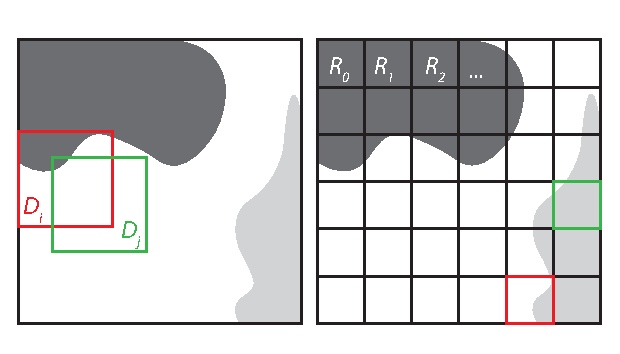
\includegraphics[width=\textwidth]{papers/ifs/images/FIC}
	\caption{Domain-, und Range-Block Paare in Grün und Rot}
	\label{ifs:FIC}
\end{figure}

\subsubsection{Rekonstruktion des Bildes}
Mit den gefundenen Abbildungen lässt sich das Bild generieren.
Wir beginnen wie schon im letzten Kapitel mit einer beliebigen Startmenge.
In unserem Fall ist dieses ein Bild  $f_0$ derselben Grösse.
Nun ersetzen wir jedes $R_i$ mit der Transformierten des zugehörigen Domain-Blocks $T(G_j)$.
Dies wird verkürzt als Operator $W$ geschrieben.
So erhalten wir ein neues Bild $f_1 = W(f_0)$.
Dieses Vorgehen führen wir iteriert aus bis wir von $f_n = W(f_{n-1})$ zu $f_{n-1}$ kaum mehr einen Unterschied feststellen. Die Iteration hat nun ihren Attraktor, das Bild, erreicht.

\subsubsection{Farbbilder}
Dieses Verfahren mit Graustufenbilder lässt sich ganz einfach auf Farbbilder erweitern.
Jeder Pixel eines Farbbildes besteht aus einem Rot, Grün und Blauwert (RGB).
Teilt man ein Bild in die drei Farbkanäle auf, das heisst, es wird nur noch ein Farbwert benutzt, erhält man drei Bilder, welche wie ein Graustufenbild sind.
Nun wendet man auf jeden dieser Farbkanalbilder den Algorithmus an, und fügt nach der Rekonstruktion die Kanäle wieder zusammen. 

\subsubsection{Performance des Verfahren}
Experimentelle Beobachtungen haben gezeigt, dass dieser Grundalgorithmus der fraktalen Bildkompression recht langsam ist und auch schlecht für grössere Bilder skaliert.
Man kann die Laufzeit zwar verbessern indem man die Domain-Blöcke auch disjunkt macht, und für weniger detailreiche Bilder ein grösseres $b$ wählt, jedoch wird er auch so nicht so schnell wie zum Beispiel das JPEG-Verfahren.
Es wurden bessere Algorithmen der fraktalen Bildkompression entwickelt, doch auch diese können, vor allem in der Laufzeit, noch nicht mit herkömmlichen Komprimierungsverfahren mithalten.

\subsection{Beispiel}
Wir verwenden dafür den oben beschriebenen Algorithmus, welcher uns für jeden Range-Block die benötigten Parameter liefert.
Mit diesen lässt sich das Bild im Anschluss wieder Rekonstruieren.
Die Range-Blöcke wurden $4\times4$ gewählt und die Domain dementsprechend $8\times8$.
Um etwas Zeit bei der Komprimierung zu ersparen, wurden nur disjunkte Domain-Blöcke gebraucht.
Als erstes Beispiel wählen wir das 360$\times$360 Pixel Bild von Rapperswil in Abbildung \ref{ifs:original}.
Das Startbild ist ein mittelgraues 360$\times$360 Pixel Bild, Abbildung \ref{ifs:bild0}.
Es kann jedoch ein beliebiges Startbild sein.
Nun lassen wir das PIFS laufen.
Wie wir in Abbildung \ref{ifs:rappirecoa} sehen, ist schon nach der ersten Iteration das Bild schon erkennbar.
Nach der fünften Iteration, Abbildung \ref{ifs:rappirecoc} gibt es fast keinen Unterschied mehr zur letzten Iteration, wir können die Rekonstruktion beenden.
\begin{figure}	
	\centering
	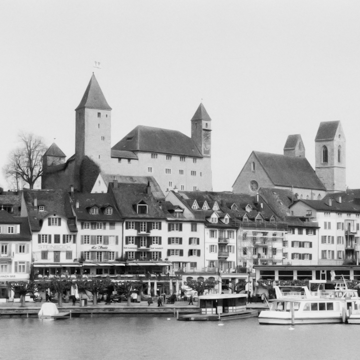
\includegraphics[width=0.4\textwidth]{papers/ifs/images/original}
	\caption{Original Bild von Rapperswil}
	\label{ifs:original}
\end{figure}
\begin{figure}
	\centering
	
\includegraphics[width=0.4\textwidth]{papers/ifs/images/rapperswil}
	\caption{Startbild}
	\label{ifs:bild0}
\end{figure}

\begin{figure}
	\centering
	\subfigure[]{
		\label{ifs:rappirecoa}
		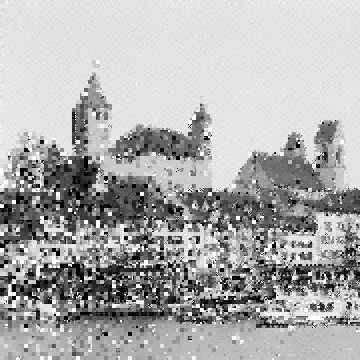
\includegraphics[width=0.32\textwidth]{papers/ifs/images/rapperswil01}}
	\subfigure[]{
		\label{ifs:rappirecob}
		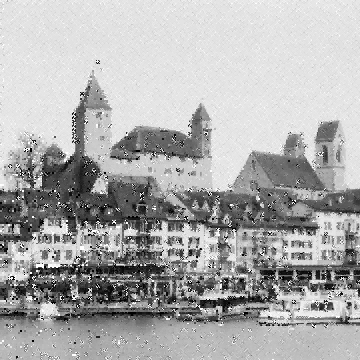
\includegraphics[width=0.32\textwidth]{papers/ifs/images/rapperswil001}} 
	\subfigure[]{
		\label{ifs:rappirecoc}
		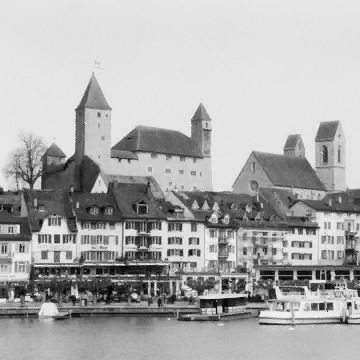
\includegraphics[width=0.32\textwidth]{papers/ifs/images/rapperswil04}}
	\caption{(a) 1. Iteration (b) 2. Iteration (c) 5. Iteration}
		\label{ifs:rappireco}
\end{figure}
